\chapter{Literature Review}

\section{Background}

Storing and verifying students' academic transcripts can be costly and time-consuming for academia, students and businesses alike. Through this project, we look to turn to blockchain technology for a solution. But first of all, let us start with a review of the blockchain technology and its current applications.\\\\
Bitcoin which is a peer to peer electronic cash system was revealed to the world in 2008 by Satoshi Nakamoto whose identity is still unknown and was offered to the open source community in 2009. The decentralised nature of the technology used by bitcoin came to be known as blockchain.\\
\begin{figure}[!h]
\centering
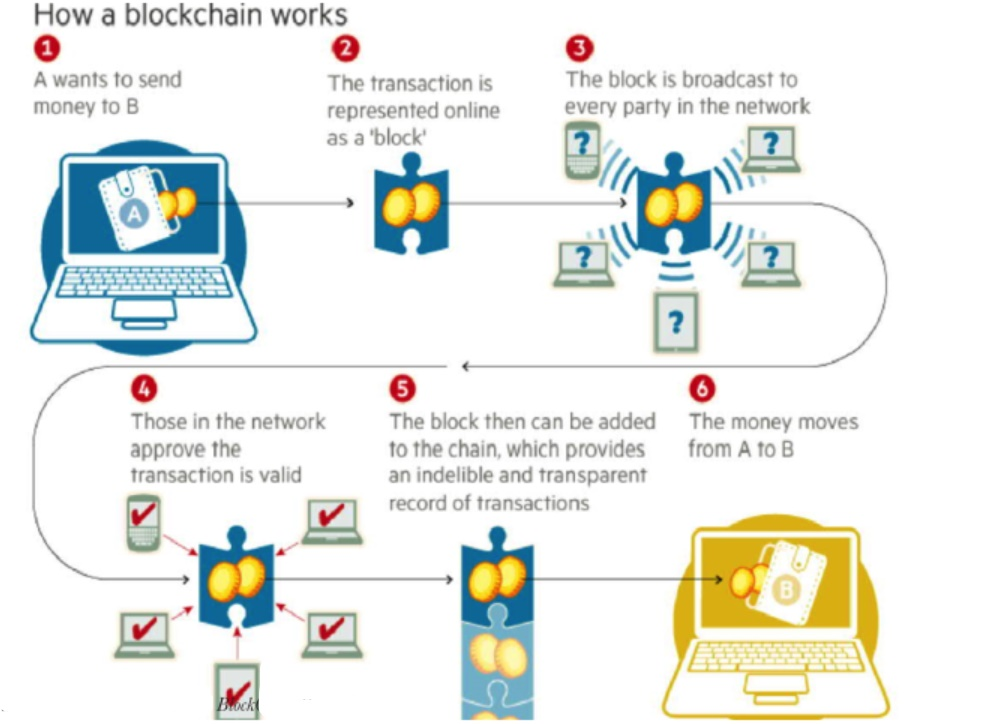
\includegraphics[scale=0.3]{images/howitworks.jpg}
\caption{How blockchain works (Applied Innovation Review, Issue No.2 - June 2016)}
\end{figure}
Bitcoin uses cryptographic proof instead of the trust-in-the-third-party mechanism for two willing parties to execute an online transaction over the Internet.\\
Each transaction is protected through a digital signature, is sent to the “public key” of the receiver, and is digitally signed using the “private key” of the sender. In order to spend money, the owner of the cryptocurrency needs to prove his ownership of the “private key”.\\
The entity receiving the digital currency then verifies the digital signature, which implies ownership of the corresponding “private key”, by using the “public key” of the sender on the respective transaction.\\
Each transaction is broadcasted to every node in the Bitcoin network and is then recorded in a public ledger after verification. Every single transaction needs to be verified for validity before it is recorded in the public ledger.\\\\
\subsubsection{Storing documents on the blockchain}
Up until 2014, blockchain did not seem to have much potential independent of bitcoin. In 2014, some people realised other potential uses of blockchain in disciplines like supply chain, healthcare, insurance, education among others.\\
Over the past several years, there has been a keen interest in how we can use blockchains for storing documents.\\
There are two main ways to store a document on the blockchain. One option is to store the entire document itself on-chain. Alternatively, one can store a hash of it on the blockchain.
\begin{itemize}
\item \textbf{Storing Entire Document} - Storing a whole document on-chain is possible with certain blockchains.\\
However, we found out that it is rarely a good idea because of something called access latency. Fully decentralized public blockchains have thousands of nodes and this means it takes long for network users to upload and download files, such as documents. 
\item \textbf{Storing a Hash} - This method involves storing a document’s hash on-chain while keeping the whole document elsewhere. The document could be stored in a centralized database or on a distributed file storage system. The document can be put through a secure hash algorithm like SHA-256 and then the hash is stored in a block. We find this to be the most efficient method as it saves a huge amount of space and cost. Additionally, using the hash, one is able to tell if someone tampers with the original document.
\end{itemize}
There are few projects that focus on documents alone right now. Most are built around decentralized file storage, which includes documents.\\\\
One project that is focused specifically on documents, particularly signed documents, is Blocksign\cite{art6}. This uses the hash method. A user will sign the document and send it to Blocksign, where it is then hashed, and the hash is stored on the Bitcoin blockchain.\\\\
Other cryptocurrency projects designed for decentralized storage more generally include Siacoin, Storj and Cryptyk.\\\\
\textbf{Siacoin}\cite{art7} - uses their distributed network to store an encrypted version of one`s document. The Siacoin network is comprised of hosts who provide storage and clients who desire storage. Clients and hosts agree upon contracts detailing the commitments made by the storage providers. Sia`s own proof of work blockchain stores these contracts.\\\\
\textbf{Storj}\cite{art8} - runs atop the Ethereum\cite{art9} blockchain. A hash of the document is stored within a hash table on-chain. Additionally, its distributed network also stores your document.\\\\
\textbf{Cryptyk}\cite{art10} - an enterprise-focused platform to store documents, uses a blockchain more distantly than all of the above	. You do not store any documents or hashes on-chain. Instead, a distributed cloud system stores the documents. The platform only uses a blockchain to manage and referee document access and sharing.\\\\
Described below are not only some of the contributions, but also weaknesses and gaps that are associated with this technology.
\subsubsection{Contributions}
Because decentralized applications run on the block chain, they benefit from all of its properties, which include:-\\
\begin{itemize}
\item \textbf{Immutability} – A third party cannot make any changes to data.
\item \textbf{Corruption \& tamper proof} – Apps are based on a network formed around the principle of consensus, making censorship impossible.
\item \textbf{Secure} – With no central point of failure and secured using cryptography, applications are well protected against hacking attacks and fraudulent activities.
\item \textbf{Zero downtime} – Apps never go down and can never be switched off.
\end{itemize}
For an example of the contribution of this technology, we look at the University of Nicosia in Cyprus, which is using the technology to record students' achievements. According to George Papageorgiou, a digital currency lecturer at the university, the technology is proving popular. He had this to say to CNBC News: \\ 
\textit{"We've only encountered enthusiasm in the practical uses so far and students are glad to be able to verify, with their new knowledge and the blockchain, that their digital certificate is genuine and that it cannot be recreated.\\
We believe this instills confidence in both students and potential employers that (they) can check on their own, whether a presented certificate is real or not"}.\cite{art11} \\ \\
This is proof that the implementation is already reaping fruits in some institutions around the world.

\subsubsection{Weaknesses and gaps}

However, despite all the possibilities offered by blockchain, there have been various challenges associated with it.\\\\
We observe challenges in both the perspective of the end-user, and we, the researchers. From the user’s view, according to Donald Clark \cite{art12}, an EdTech entrepreneur and advisor of EdTech companies, some public sector organizations just don’t like the innovation and stick to their institutional silos. This is basically because the technology has not been around for a long time which makes many potential users have doubts about its possibilities. To overcome this, we intend to train the parties in these institutions on how to use this technology and also show them the advantages.\\\\
From our research perspective, the major challenge is that the subject of study is of a relatively early stage. Blockchain technologies are under active development globally, and there may be recent advances that impact our findings.\\\\
In conclusion, it is important to note that blockchain is a technology that clearly has applications in the world of learning at individual, institutional and international levels. It is relevant in all sorts of contexts: schools, colleges, universities among others.\\\\
One thing we know for sure is that students have their eyes open and are looking for alternatives. Perhaps, like Bitcoin, the blockchain revolution will ultimately come from left of field.
\newpage

